\chapter{Fixed Wind sUAS Development}
\label{chap:Fixed_Wing}

\section{Range \& Endurance}
The fixed wing sUAS we used for this project was the Aerosonde UAV. The parameters as given for the Aerosonde UAV are in the Figure below.

\subsection{Range}
The range of an aircraft is technically defined as the total distance measured with respect to the ground traversed by the aircraft on one full tank of fuel. It is used to estimate engine performance in terms of fuel consumption. The maximum total range is the maximum distance an aircraft can fly between takeoff and landing, as limited by fuel capacity in powered aircraft, or cross-country speed and environmental conditions in unpowered aircraft. In this project, the maximum range of the given aircraft is calculated with respect to the propeller data obtained from the UIUC database for the given propeller (APC 16X8).

In order to calculate the range of the aircraft with respect to the different powertrain systems, the following specifications are adopted:

\begin{enumerate}
	\item \textbf{Specific Fuel Consumption (SFC) (for propeller)} : Specific fuel consumption is one of the important metrics in determining the performance of a propeller-driven aircraft. SFC is defined as the weight of the fuel consumed by the reciprocating engine per unit power per unit time.
	
	\item \textbf{Thrust specific fuel consumption (TSFC) (for jet engine)} : The thrust specific fuel consumption of a jet engine is defined as the fuel efficiency of an engine design with respect to thrust output. TSFC is the mass of fuel burned by an engine in one hour divided by the thrust that the engine produces.
\end{enumerate}

The maximum range for the APC 16X8 propeller is calculated using the given formula: 

\begin{equation}
R = \int_{W_0}^{W_1} \frac{\eta}{c_p} \frac{C_L}{C_D} \frac{dW}{W} = \frac{\eta}{c_p} \frac{C_L}{C_D} ln(\frac{W_0}{W_1})	
\end{equation}

\begin{equation}
	R_{max} = \frac{\eta}{c_p} \frac{C_L}{C_D} ln(\frac{W_0}{W_1}) = \frac{\eta/c_p}{2\sqrt{KC_{D_0}}}ln(\frac{W_0}{W_1})	
\end{equation}

\begin{figure}
	\centering
	\includegraphics[width=0.8\textwidth]{Images/Fixed_Wing_parameters}
	\caption{Given Parameters}
	\label{fig:Parameters}
\end{figure}

\textbf{Note :} To cover the longest distance, common sense says that we must use the minimum fuel consumption per unit distance (e.g., km or mile).

\subsection{Endurance}

The endurance of an aircraft is defined as the total time that an aircraft stays in the air on a tank of fuel. Like the range characteristics, to achieve maximum endurance, it is advised to use the minimum thrust per unit time. For a steady level flight, the lift is equal to weight and the thrust is equal to the drag (L = W, T = D). 

To calculate the maximum endurance for a propeller-driven aircraft, the following parameters are required :

\begin{enumerate}
	\item Maximum weight loss (Wf = W0 – W1)
	\item Maximum $ C_l^\frac{3}{2}/C_d $
\end{enumerate}

The maximum endurance for a propeller-driven aircraft is calculated using the given formula :

\begin{equation}
	E = \int_{W_0}^{W_1} \frac{\eta}{c_p V}\frac{C_L}{C_D}\frac{dW}{W} 
\end{equation}

\begin{equation}
	 = \int_{W_0}^{W_1} \frac{\eta}{c_p}\sqrt{\frac{\rho S}{2}}\frac{C_L^{1.5}}{C_D}\frac{dW}{W^{1.5}} 
\end{equation}

\begin{equation}
	E = \frac{\eta}{c_p}\sqrt{2\rho S}(\frac{C_L^{1.5}}{C_D})(\frac{1}{\sqrt{W_1}} - \frac{1}{\sqrt{W_0}}) 
\end{equation}

Based on the above-mentioned procedures, the results of the multi-rotor drone (quadcopter) are as follows:

Max. Range = 390.04 kms

Max. Endurance = 5.88 hours

\section{Fixed Wing Aircraft Dynamics}
We are using the Linearized Models in the \cite{Randal2012} for Developing the Flight Dynamics for the Fixed Wing Aircraft. The Aircraft Dynamics is primarily divided into two different parts, The Longitudinal Dynamics and the Lateral Dynamics. The Linearized Equations are demonstrated in the State Space Models as given in the further subsections. The Longitudinal Dynamics has the elevator and the thrust as the inputs. The elevator controls the pitching and the thrust controls the Speed. The Lateral Dynamics has the aileron and the rudder as the inputs.


\subsection{Longitudinal Flight Dynamics}
The Longitudinal Dynamics has 6 states, u, w, q, $\theta$, h. The Longitudinal Statespace can be seen as below. The Longitudinal The Dynamics Equations for all these states are linearized using Taylor's sequence at the Equilibrium Locations. We calculate the Equilibrium values using the non-linear Dynamic Equations.

Given a nonlinear system described by the differential equations
$$
\dot{x}=f(x, u),
$$
where $f: \mathbb{R}^{n} \times \mathbb{R}^{m} \rightarrow \mathbb{R}^{n}, x$ is the state of the system, and $u$ is the input, the system is said to be in equilibrium at the state $x^{*}$ and input $u^{*}$ if
$$
f\left(x^{*}, u^{*}\right)=0 .
$$

When an Aircraft is in constant-altitude, wings-level steady flight, a subset of its states are in equilibrium. In particular, the altitude h; the body frame velocities u, v, w; the Euler angles $\phi$, $\theta$, $\psi$; and the angular rates p, q, and r are all constant, Zero in this case. 

The final state-Space Equation is as given below \\\

\begin{aligned}
	&\left(\begin{array}{c}
		\dot{\bar{u}} \\
		\dot{\bar{w}} \\
		\dot{\bar{q}} \\
		\dot{\bar{\theta}} \\
		\dot{\bar{h}}
	\end{array}\right)=\left(\begin{array}{ccccc}
		X_{u} & X_{w} & X_{q} & -g \cos \theta^{*} & 0 \\
		Z_{u} & Z_{w} & Z_{q} & -g \sin \theta^{*} & 0 \\
		M_{u} & M_{w} & M_{q} & 0 & 0 \\
		0 & 0 & 1 & 0 & 0 \\
		\sin \theta^{*}-\cos \theta^{*} & 0 & u^{*} \cos \theta^{*}+w^{*} \sin \theta^{*} 0
	\end{array}\right)\left(\begin{array}{c}
		\bar{u} \\
		\bar{w} \\
		\bar{q} \\
		\bar{\theta} \\
		\bar{h}
	\end{array}\right)\\
	&+\left(\begin{array}{cc}
		X_{\delta_{e}} & X_{\delta_{t}} \\
		Z_{\delta_{e}} & 0 \\
		M_{\delta_{e}} & 0 \\
		0 & 0 \\
		0 & 0
	\end{array}\right)\left(\begin{array}{l}
		\bar{\delta}_{e} \\
		\bar{\delta}_{t}
	\end{array}\right)
\end{aligned} \\\\

The Coefficients of the Matrix are as given below: \\\
\begin{lstlisting}
	
Cxo = -P.CDo*cos(alpha) + P.CLo*sin(alpha)
Cxa = -P.CDa*cos(alpha) + P.CLa*sin(alpha)
Cxq = -P.CDq*cos(alpha) + P.CLq*sin(alpha)
Cxdelta_e = -P.CDdelta_e*cos(alpha) + P.CLdelta_e*sin(alpha)

Xu  = (2*qs*Cxo - rho*Sprop*Ue*C_T)/m
Xw  = Cxa*qs/m
Xq  = Cxq*qs1*c_bar/(2*m)
Xdelta_e = Cxdelta_e*qs1_2/m
Xdelta_t = (rho*Sprop*C_T*k^2)/m

Czo = -P.CLo*cos(alpha) - P.CDo*sin(alpha)
Cza = -P.CLa*cos(alpha) - P.CDa*sin(alpha)
Czq = -P.CLq*cos(alpha) - P.CDq*sin(alpha)
Czdelta_e = -P.CLdelta_e*cos(alpha) - P.CDdelta_e*sin(alpha)

Zu  = 2*qs*Czo/m
Zw  = Cza*qs/m
Zq  = Ue + Czq*qs1*c_bar/(2*m)
Zdelta_e = Czdelta_e*qs1_2/m

Mu  = 2*qs*c_bar*Cmo/Iyy
Mw  = Cma * qs * c_bar/Iyy
Mq  = Cmq*qs1*c_bar*c_bar/(2*Iyy)
Mdelta_e = Cmdelta_e*qs1_2*c_bar/Iyy
\end{lstlisting}\\\

\subsection{Lateral Flight Dynamics}
For the lateral dynamics, the variables of interest are the roll angle $\phi$, the
roll rate p, the heading angle $\psi$, and the yaw rate r. The control surfaces
used to influence the lateral dynamics are the ailerons $\delta_{a}$, and the rudder
$\delta_{r}$ . The ailerons are primarily used to influence the roll rate p, while the
rudder is primarily used to control the yaw $\psi$ of the aircraft.\\\

\begin{aligned}
	\left(\begin{array}{c}
		\dot{\bar{v}} \\
		\dot{p} \\
		\dot{\bar{r}} \\
		\dot{\bar{\phi}} \\
		\dot{\bar{\psi}}
	\end{array}\right)=&\left(\begin{array}{ccccr}
		Y_{v} & Y_{p} & Y_{r} & g \cos \theta^{*} \cos \phi^{*} & 0 \\
		L_{v} & L_{p} & L_{r} & 0 & 0 \\
		N_{v} & N_{p} & N_{r} & 0 & 0 \\
		0 & 1 & \cos \phi^{*} \tan \theta^{*} & q^{*} \cos \phi^{*} \tan \theta^{*}-r^{*} \sin \phi^{*} \tan \theta^{*} & 0 \\
		0 & 0 & \cos \phi^{*} \sec \theta^{*} & p^{*} \cos \phi^{*} \sec \theta^{*}-r^{*} \sin \phi^{*} \sec \theta^{*} & 0
	\end{array}\right) \\
	& \times\left(\begin{array}{c}
		\bar{v} \\
		\bar{p} \\
		\bar{r} \\
		\bar{\phi} \\
		\bar{\psi}
	\end{array}\right)+\left(\begin{array}{cc}
		Y_{\delta_{a}} & Y_{\delta_{r}} \\
		L_{\delta_{a}} & L_{\delta_{r}} \\
		N_{\delta_{a}} & N_{\delta_{r}} \\
		0 & 0 \\
		0 & 0
	\end{array}\right)\left(\begin{array}{c}
		\bar{\delta}_{a} \\
		\bar{\delta}_{r}
	\end{array}\right)
\end{aligned} \\\\

The Coefficients of the Matrix are as given below: \\\

\begin{lstlisting}
	
	Yv = 2*Cyo*qs/m + qs*Cyb/m
	Yp = Cyp*qs1*b/(2*m)
	Yr = -Ue + (Cyr*qs1*b/(2*m))
	Ydelta_a = Cydelta_a*qs1_2/m
	Ydelta_r = Cydelta_r*qs1_2/m
	
	Lv = Cpb*qs*b
	Lp = Cpp*qs1*b^2/2
	Lr = Cpr*qs*b^2/2
	Ldelta_a = Cpdelta_a * qs1_2 * b
	Ldelta_r = Cpdelta_r * qs1_2 * b
	
	Nv = Crb * qs * b
	Np = Crp * qs1 * b^2 / 2
	Nr = Crr * qs1 * b^2 / 2
	Ndelta_a = Crdelta_a * qs1_2 * b
	Ndelta_r = Crdelta_r * qs1_2 * b
\end{lstlisting} \\\

\section{Simulink Model}
The Given State-Space setup was implemented in Matlab with a Level2 S Function Block. The Block takes 4 inputs in the following order : $\delta_{e}$, $\delta_{a}$, $\delta_{r}$, $\delta_{t}$. The Block further provides 12 outputs, giving the state for both the longitudinal and lateral Systems. The complete Simulink Model can be seen in the figure \ref{fig:fixed_wing_simulink}.\\

The Simulink model performs all the three manuevers in the order provided in the Queation. The input for the system is controlled from the refernece position subsystem, which gives out 5 outputs, height h, $\psi$, $\phi$, V, U. The error are calculated using feedback loops and are further fed to PIDs. A Radian to Degree converter is used in $\phi$ and $\psi$  as the outputs are in Radians. The reference position subsystem is time-based with a digital clock as an input and time based if-else block. We calculated the time for each manuever and used the digital clock to change the input for the positions. 

\begin{figure}
	\centering
	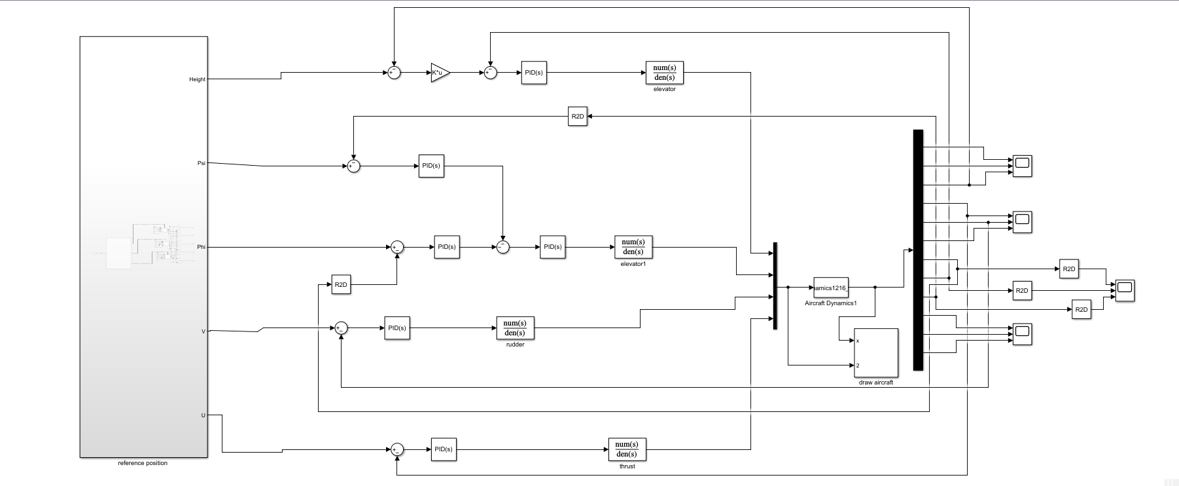
\includegraphics[width=1\textwidth]{Images/fixed_wing_simulink}
	\caption{Simulink Model}
	\label{fig:fixed_wing_simulink}
\end{figure}

